    \documentclass[a4paper,11pt]{article}
    \usepackage[german,italian]{babel}
    \usepackage{fancyhdr}


    \textwidth16cm \textheight24cm \topmargin0mm \headheight0mm
    \headsep5mm \oddsidemargin0mm \evensidemargin0mm
    \parindent0mm


    \usepackage{amsmath}
    \usepackage{parskip}
    \usepackage{dsfont}
    \usepackage{fullpage}
    \usepackage{amssymb}
    \usepackage{tikz,pgfplots}
    \usepackage{cancel}
    \usepackage{lmodern}

    \usepackage[T1]{fontenc}

    \usepackage{theorem}
    \usepackage{psfrag}
    \usepackage{color}
    \usepackage{graphicx}
    \usepackage{hyperref}

    \usepackage{background}
    \usepackage{keystroke}
    \usepackage{etoolbox}

    \usepackage{physics,bm}

    \usepackage[outline]{contour} % glow around text
    \usetikzlibrary{angles,quotes} % for pic (angle labels)
    \usetikzlibrary{decorations.markings}
    \usetikzlibrary{shapes} % for path name
    \tikzset{>=latex} % for LaTeX arrow head
    \contourlength{1.4pt}

    \usepackage{xcolor}
    \colorlet{Ecol}{orange!90!black}
    \colorlet{EcolFL}{orange!90!black}
    \colorlet{veccol}{green!45!black}
    \colorlet{EFcol}{red!60!black}
    \tikzstyle{charged}=[top color=blue!20,bottom color=blue!40,shading angle=10]
    \tikzstyle{darkcharged}=[very thin,top color=blue!60,bottom color=blue!80,shading angle=10]
    \tikzstyle{charge+}=[very thin,top color=red!80,bottom color=red!80!black,shading angle=-5]
    \tikzstyle{charge-}=[very thin,top color=blue!50,bottom color=blue!70!white!90!black,shading angle=10]
    \tikzstyle{darkcharged}=[very thin,top color=blue!60,bottom color=blue!80,shading angle=10]
    \tikzstyle{gauss surf}=[green!70!black,top color=green!2,bottom color=green!80!black!70,shading angle=5,fill opacity=0.6]
    \tikzstyle{gauss lid}=[gauss surf,middle color=green!80!black!20,shading angle=40,fill opacity=0.7]
    \tikzstyle{gauss dark}=[green!60!black,fill=green!60!black!70,fill opacity=0.8]
    \tikzstyle{gauss line}=[green!80!black]
    \tikzstyle{gauss dashed line}=[green!60!black!80,dashed,line width=0.2]
    \tikzstyle{vector}=[->,thick,veccol]
    \tikzstyle{normalvec}=[->,thick,blue!80!black!80]
    \tikzstyle{EField}=[->,thick,Ecol]
    \tikzstyle{EField dashed}=[dashed,Ecol,line width=0.6]
    \tikzset{
    EFieldLine/.style={thick,EcolFL,decoration={markings,
                        mark=at position #1 with {\arrow{latex}}},
                        postaction={decorate}},
    EFieldLine/.default=0.5}
    \tikzstyle{measure}=[fill=white,midway,outer sep=2]
    \def\L{2.2}
    \def\H{2.2}
    \def\offset{2.0}
    \def\W{0.30}
    \def\Nx{5}
    \def\Ny{5}













    \makeatletter
    \patchcmd{\tableofcontents}{\@starttoc{toc}}{\hypertarget{totoc}{}\@starttoc{toc}}{}{}
    \makeatother

    \SetBgScale{1}
    \SetBgAngle{0}
    \SetBgColor{black}
    \SetBgPosition{current page.south}
    \SetBgVshift{20pt}
    \SetBgContents{\tikz[remember picture,overlay]
        \node[inner sep=0pt] {\hyperlink{totoc}{\Return}};}

    \hypersetup{
        colorlinks=true,
        linkcolor=black,
        urlcolor=blue,
        pdftitle={Elettricità},
        pdfpagemode=FullScreen,
    }




    \begin{document}




    \title{Fisica}

    \author{Massimiliano Ferrulli}
    \date{21.04.2022}



    \maketitle

    \section*{Elettricità}
    Capitoli sulla legge di Coulomb e dei campi elettrici

    \pagebreak
    \tableofcontents
    \pagebreak

\section{Conduttori}
ci sono 4 tipi di conduttori:
\\
I conduttori sono sostanze attraverso cui le cariche si muovono liberamente
\\
I superconduttori permettono alle cariche di muoversi al loro interno senza alcun ostacolo
\\
I semiconduttori manifestano un comportamento intermedio tra conduttori e isolanti
\\
Gli isolanti sono sostanze che non permettono alle cariche di muoversi liberamente

\section{Legge di Coulomb}
l'equazione della forza elettrostatica è (applicabile solamente per cariche puntiformi o racchiuse in particelle):
\begin{center}
    \[
    F_e = \frac{1}{4\pi \epsilon_0}\frac{q_1 q_2}{r^2} \, \, \,  \text{oppure} \, \, \, F_e = k  \frac{q_1 q_2}{r^2}
    \]
\end{center}
questo è il modulo della forza e \( \varepsilon_0\) è la costante dielettrica nel vuoto

\section{Campo Elettrico}

il campo elettrico è un campo vettoriale, possiamo definire \textbf{E} per ciascun punto dello spazio attorno ad una carica.
\\
attraverso una carica esplorativa \(q_0\) possiamo misurare la forza elettrostatica \textbf{F} che agisce su di essa, a patto che la carica \(q_0\) sia piccola a sufficienza per non perturbare la distribuzione. 
\begin{center}
    \[
    E = \frac{F}{q_0^+}
    \]
\end{center}
esempio di campo elettrico con l'illustrazione delle sue linee di campo:
\begin{center}
    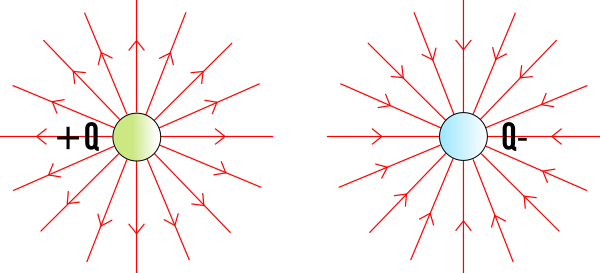
\includegraphics[scale=0.5]{linee-di-campo-elettrico-di-una-carica-puntiforme.png}
\end{center}
\pagebreak
esempio di campo elettrico generato da un dipolo elettrico:
\begin{center}
    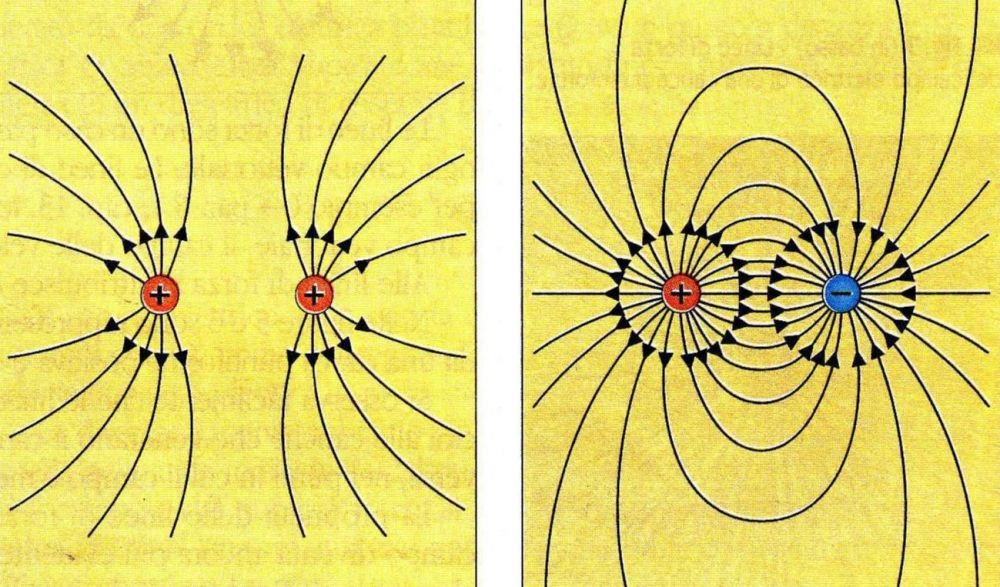
\includegraphics[scale=0.35]{linee_di_forza_di_un_dipolo_elettrico.jpg}
\end{center}

ora vogliamo calcolare il campo elettrico generato da varie geometrie:
\\
\subsection{Bacchetta curva}
Campo elettrico generato da una bacchetta curva a condizione che sia una bacchetta isolante e sottile a tal punto da non considerare lo spessore
\begin{align*}
    \lambda = \frac{q}{L} \hspace{5mm} dq = \lambda ds 
    \\
    dF_e = \frac{1}{4\pi\varepsilon_0} \frac{Q\lambda ds}{r^2} 
    \\
    dF_x = dF * cos(\alpha) \hspace{3mm} \alpha \in [0;\frac{\pi}{k}]
\end{align*}

\begin{align*}
    F = \frac{2}{4 \pi \varepsilon_0} \frac{Q \lambda}{r} \int_{0}^{\frac{\pi}{k}} cos(\alpha) \,d\alpha 
    \\
    \text{oppure}
    \\
    F = \frac{1}{4 \pi \varepsilon_0} \frac{Q \lambda}{r} \int_{-\frac{\pi}{k}}^{\frac{\pi}{k}} cos(\alpha) \,d\alpha 
    \\
    E = \frac{F}{Q} = \frac{1}{4 \pi \varepsilon_0} \frac{ \lambda}{r} \int_{-\frac{\pi}{k}}^{\frac{\pi}{k}} cos(\alpha) \,d\alpha 
\end{align*}

\pagebreak
\subsection{Anello}
Campo elettrico generato da un anello a condizione che sia una bacchetta isolante e sottile a tal punto da non considerare lo spessore
\begin{center}
    \begin{tikzpicture}[x={(1,0)},y={(0,0.5)}]
    \def\r{1.3}
    \def\dr{0.53}
    \def\dtu{5}   % upper angle dq segment
    \def\dtd{-15} % lower angle dq segment
    \def\Ex{0.6}
    \def\Ey{1.1}
    \def\N{10}
    \coordinate (O) at (0,0);
    \coordinate (P) at (0,4.0);
    \coordinate (Y) at (0,6.0);
    \coordinate (-Y) at (0,-3.0);
    \coordinate (R) at (\r,0);
    
    % PLANE
    \draw[thick] (O) -- (-Y); % axis below
    \draw[charged,even odd rule]
      (O) circle (\r+\dr) circle (\r);
    \draw[darkcharged]
      (O) ++ (\dtu:\r) arc (\dtu:\dtd:\r) to[out=60,in=100]++ (\dtd:\dr) arc (\dtd:\dtu:\r+\dr) to[out=130,in=60] cycle;
    \foreach \i [evaluate={\cang=3+\i*360/\N;}] in {1,...,\N}{
      \node[scale=0.9,rotate=0] at (\cang:\r+\dr/2) {$+$};
    }
    
    % CHARGE
    %\node[below=1,right=0,scale=1.0] at (4:\r+\dr) {$\dd{q} = \lambda \dd{x} = \lambda r\dd{\theta}$};
    \node[below=10,right=0,scale=1.0] at (4:\r+\dr) {
      $\begin{aligned}
         \dd{q} &= \lambda \dd{s}\\
                
      \end{aligned}$
    };
    
    % AXIS
    \draw[->,thick] (O) -- (Y) node[above] {$y$};
    
    % VECTORS
    \draw[EField,very thick] (P) --++ ( 0.0,\Ey) node[right=1] {$\dd{\vb{E}_y}$};
    \draw[EField,very thick] (P) --++ (-\Ex,0.0) node[left=2] {$\dd{\vb{E}_x}$};
    \draw[EField,very thick] (P) --++ (-\Ex,\Ey) node[above left=-2] {$\dd{\vb{E}}$};
    \draw[EField,-,dashed,thin] (P) ++ (0,\Ey) --++ (-\Ex,0) --++ (0,-\Ey);
    \node[fill=blue!60!black,circle,inner sep=1.1] (P') at (P) { };
    \node[above=3,right=1] at (P') {P};
    \draw[vector,veccol] (R) -- (P') node[midway,above=5] {$\vb{r}$};
    \draw[<->] (0,0) --++ (0:\r) node[midway,above] {$R$};
    \draw[blue,very thick] (0,0) -- (P) node[midway,left=3] {$\vb{z}$};
    
\end{tikzpicture}

\end{center}

\begin{align*}
     dF_y = dF \cos(\theta) =& \frac{1}{4 \pi \varepsilon_0} \frac{Q \lambda ds}{r^2} \cos(\theta)
     \\
     r^2 = R^2 + z^2 \hspace{5mm} &\cos(\theta) = \frac{z}{r} 
     \\
     dF_y = \frac{1}{4 \pi \varepsilon_0} \frac{Q \lambda ds}{R^2 + z^2} \frac{z}{r}  =& \frac{1}{4 \pi \varepsilon_0} \frac{Q \lambda ds z}{(R^2 + z^2)^\frac{3}{2}}
\end{align*}

    \begin{align*}
        F = \int dF_y = \frac{Q \lambda z}{4 \pi \varepsilon_0 (R^2 + z^2)^\frac{3}{2}} \int_{0}^{2\pi r}  \,ds 
        \\
        E = \frac{F}{Q} = \frac{ \lambda z}{4 \pi \varepsilon_0 (R^2 + z^2)^\frac{3}{2}} \int_{0}^{2\pi r}  \,ds
    \end{align*}


\end{document}


